
% Intolerance of ambiguity is the sign of an authoritarian personality.


%\documentclass[natbib]{svjour3}
%\documentclass[manuscript]{acmart}
%\documentclass[10pt,journal,compsoc]{IEEEtran}
%\documentclass{sig-alternate}
\documentclass{llncs}

\usepackage{booktabs} % For formal tables
\usepackage[T1]{fontenc}
\usepackage[]{hyperref} %sections as bookmarks in adobe pdf
%\hypersetup{pdfpagelabels=false}
\hypersetup{
	colorlinks = true, %Colours links instead of ugly boxes
	urlcolor   = blue, %Colour for external hyperlinks
	linkcolor  = blue, %Colour of internal links
	citecolor  = blue   %Colour of citations
}

\usepackage{times}
\usepackage{multirow}
\usepackage{wrapfig}
%\usepackage[usenames, dvipsnames]{color}


% Macros for proof-reading & corrections
\usepackage[normalem]{ulem} % for \sout
\usepackage{xcolor,xspace}
% Put edit comments in a really ugly standout display
\usepackage{ifthen}

% Advanced Math
\usepackage{amsmath}
%\usepackage{amssymb}	% double line font letters (for number sets N,Z,D,Q,R)

% Images and Floats
\usepackage{epsfig}
%\usepackage{epstopdf}

%\usepackage{caption}
%\usepackage{subcaption}

%\usepackage{enumitem}
\usepackage{graphicx,wrapfig,lipsum}
\usepackage{flushend}



%For code listings:
\usepackage{listings}
\usepackage{parcolumns}
%\usepackage[sectionbib,square]{natbib}


%\setlength{\paperheight}{11in}
%%%%%%%%%%%%%%%%%%%%%%%%%%%%%%%%%%%%%%%%%%%%%




% Standard shortcuts
\newcommand{\eg}{\emph{e.g.,~}}							% exempli gratia (for the sake of example)
\newcommand{\ie}{\emph{i.e.,~}}							% id est (that is)
\newcommand{\Fig}[1]{Fig.~\ref{#1}}  			% choose Fig. or Figure, depending on the style
\newcommand{\Table}[1]{Table~\ref{#1}}	    % Table reference
\newcommand{\Sect}[1]{Section~\ref{#1}}	  % section name always with a capital S
\newcommand{\Model}[1]{\textsf{\small{#1}}} % name of any modeling artifact (e.g., formalism, model element, rule, ...)
\newcommand{\Code}[1]{\texttt{\small{#1}}}	% inline code
\providecommand{\e}[1]{\ensuremath{\times 10^{#1}}}	% scientific notation: x.10^y

%%%%%%%%%%%%%%%%%%%%%%%%%%%%%%%%%%%%%%%%%%%%%

% Shortcuts
\newcommand{\MOF}{\textsc{MOF}\xspace}
\newcommand{\ocl}{\textsc{OCL}\xspace}
\newcommand{\OCL}{\textsc{OCL}\xspace}
\newcommand{\nsga}{\textsc{NSGA-II}\xspace}
\newcommand{\MDE}{\textsc{MDE}\xspace}
\newcommand{\MT}{\textsc{MT}\xspace}
\newcommand{\WFR}{\textsc{WFR}\xspace}
\newcommand{\Ecore}{\textsc{Ecore}\xspace}
\newcommand{\OURNAME}{{our approach}\xspace}



\newcommand{\ra}{$\rightarrow$}
\newcommand{\la}{$\leftarrow$}
\newcommand{\ugh}[1]{\textcolor{red}{\uwave{#1}}} % please rephrase
\newcommand{\ins}[1]{\textcolor{blue}{\uline{#1}}} % please insert
\newcommand{\del}[1]{\textcolor{red}{\sout{#1}}} % please delete
\newcommand{\chg}[2]{\textcolor{red}{\sout{#1}}{\ra}\textcolor{blue}{\uline{#2}}} % please change
\newcommand{\move}[2]{\textcolor{blue}{\uwave{#1} (Move to #2)}} % please move


\newboolean{showcomments}
\setboolean{showcomments}{true} % toggle to show or hide comments
\ifthenelse{\boolean{showcomments}}
{\newcommand{\nb}[2]{
		\fcolorbox{gray}{yellow}{\bfseries\sffamily\scriptsize#1}
		{$\blacktriangleright$#2$\blacktriangleleft$}
	}
	\newcommand{\version}{\emph{\scriptsize$-$working$-$}}
}
{\newcommand{\nb}[2]{}
	\newcommand{\version}{}
}



\newcommand\eb[1]{\nb{EB}{\textcolor{red}{\textsl{#1}}}}
\newcommand\jc[1]{\nb{JC}{\textcolor{red}{\textsl{#1}}}}
\newcommand{\todo}[1]{\textbf{\textcolor{red}{TODO: #1}}}
\newcommand\syn[0]{\fcolorbox{gray}{green}{\bfseries\sffamily\scriptsize{SYN.}}}

\newcommand\bluefat[1]{$\blacktriangleright$\textcolor{blue}{\textit{#1}}$\blacktriangleleft$}
\newcommand\blue[1]{\textcolor{blue}{#1}}
\newcommand\red[1]{\textcolor{red}{#1}}

\makeatletter
\def\ughu{\bgroup \markoverwith{\lower3.5\p@\hbox{\sixly \textcolor{red}{\char58}}}\ULon}
\font\sixly=lasy6 % does not re-load if already loaded, so no memory problem.
\makeatother


\newcommand\missref[1]{\ughu{#1}~\ugh{[?]}}


\begin{document}


\title{(Not) Yet Another Metamodel For Traceability} 


\author{
Edouard R. Batot\inst{1} \and
Sebastien Gérard\inst{2} \and
Jordi Cabot\inst{1,3}
}


\authorrunning{E. R. Batot et al.}

\institute{
    Universitat Oberta de Catalunya -- \email{\{ebatot,jcabot\}@uoc.edu} \and
    CEA~LIST -- \email{sebastien.gerard@cea.fr} \and
    ICREA -- \email{jordi.cabot@icrea.cat} 
}

\maketitle

	\begin{abstract}
Traceability helps explaining the execution and evolution of software systems and it is a key input in many software engineering tasks such as program understanding, maintenance and debugging.
Several metamodels to facilitate the representation of traces and links between related
artefacts have been proposed. There exists a plethora of approaches that focus on distinct segments of the software development processes and products.
Nevertheless, we claim they lack the mechanisms to express important traceability aspects such as the quality of traces, their gradual decay, and the evidences supporting them. This affects the benefits traceability can bring to the above-mentioned tasks. 
This paper presents a more expressive traceability metamodel, covering all the missing dimensions in a single, but extensible and modular, design. This modularity facilitates the integration of our solution in other modeling languages or its partial adoption when only some specific traceability aspects are needed. Its extensibility facilitates its customization (\textit{e.g.,} in terms of the types of links and artefacts) to better cover specific domains.




%Traceability needs a common language.
%Adaptability means edition/extension of metamodel; thus no common metamodel because burden to adapt MM+tooling (trace representation + wrappers). 
%In any case, so long targeting a common language made researchers forget to pay attention to trace quality and accountability. (Two features still embryonic in SE in general).

%We propose 
%i) to disambiguate genericity and adaptability;
%ii) to put together adaptability and quality in a common language.


	\begin{keywords}
		Software Engineering, Model-Driven Development, Traceability, Metamodeling
	\end{keywords}
\end{abstract}


    %\hrulefill
    \section{Introduction} \label{sec:intro}

Traceability is the ability to trace different artefacts of a system (of systems). It is defined in the IEEE Standard Glossary of Software Engineering Terminology \cite{ieeeglossary-se} as the degree to which a relationship can be established between two or more products of the development process, especially products having a predecessor–successor or master–subordinate relationship to one another. 

The need for traceability has always been a recurrent aspect of software development. Across the years, there has been a continuous interest in developing techniques to facilitate the representation and analysis of traces and links between related artefacts. It helps explaining their execution and evolution as traces offer a different perspective on a system, arbitrary and customizable, where the relationships between elements is the most salient artefact. Traceability rises awareness on specific purposes or goals \cite{clelandhuang2014-traceability-trends-and-futurte-direction} and has been proven useful in a diverse number of software engineering challenges \cite{guo2017-semantically-enhanced-tracebility-deep-learning}. It is transient to any software maintenance effort such as change impact prediction \cite{helming2009-traceability-change-awareness,goknil2014-change-impact-analysis-for-requirement-metamodel}, debugging \cite{ko2008-whyline-debugging,aboussoror2012-Seeing-errors-trace-visualisation}, feature location \cite{dit2013informationRetrievalTraceabilityForFeatureLocation,meinicke2017-feature-traceability} or certification \cite{moy2013-DO-178C-testing} among many others~\cite{jaber2013-effect-on-maintenance}.

Importance of traceability is reflected in the production of many metamodels targeting the modeling of traceability aspects. Many of them focus on specific aspects or domains where the traceability mechanism is applied \cite{antoniol2017-traceability-grand-challenges,wohlrab2020-traceability-organization-process-culture,winkler2010-survey-traceability-and-MDE}. Metamodels flourish but their knowledge remains scattered among software engineering research fields. There is even work dedicated to the engineering of metamodels for traceability that offers a language dedicated to defining traceability metamodels \cite{drivalos2008-engineering-a-DSL-for-traceability}. Overall, we are still missing a generic metamodel for traceability that covers not only the representation of artefacts, traces and links between them but also quality aspects that can be used to interpret the relevance and integrity of traces. 

%We hypothesis that traceability has not made the buzz it deserves partly because past approaches have been addressing mainly technical limitations. As such most of traceability research remains separated from the effect that using traces may have on software products and agents.

The surge of artificial intelligence (AI) applications in software engineering makes good traceability support even more important as part of explainability mechanisms inherent to these AI applications \cite{ozkaya2020-differences-in-AI-enabled-engineering,Mikkonen2021}. And conversely, AI can also be a mechanism to infer new traces among sets of artefacts  \cite{borg2014-SmS-IR-for-traceability,guo2017-semantically-enhanced-tracebility-deep-learning}, which will need to come hand in hand with the proper explainability support, specially considering the non-deterministic nature of information retrieval algorithms. This non-deterministic nature draws in a significant degree of uncertainty about the results such algorithms may yield. Traces automatically identified show variable confidence. This dimension should be considered as a core concern to traceability.

In this sense, the contribution of this paper is the definition of Trace\textit{a}: a generic and extensible traceability metamodel integrating quality concerns (e.g. decay, confidence and explainability) in the definition of traces. The design of the metamodel favours also its adaptation to specific application domains and model-driven toolchains to open the door to a new generation of techniques (E.g., for impact analysis) that could benefit from our more expressive metamodel.


The rest of this paper is structured as follows. \Sect{sec:soa} introduces the state of the art through a comparison between a selected set of approaches addressing the modeling of traceability.
\Sect{sec:requirements} presents the limitations of current solutions through their main quality concerns. In \Sect{sec:metamodel}, we show and depict our metamodel Trace\textit{a} and display an illustrative example. We discuss about the integration of Tracea and more generally of traceability modeling into existing tooling in \Sect{sec:integration} before we conclude in \Sect{sec:conclusion}.

%Importance of traceability in SW eng. We can also mention it's more important now due to AI...

%Existing metamodels explore specific features or specific targets, or miss some important quality concerns. Quality aspects inherent to the relevance and precision of traces, as well as related to the uncertainty caused by automated trace retrieval techniques.

%Here is a generic (re)definition of traceability addressing these limitations.

%Example use cases



    %\input{sections/20_motivation}
    	\vspace{-0.4truecm}
\section{State of the art}\label{sec:soa}
	\vspace{-0.2truecm}

We have identified over 80 approaches aimed a modeling traces and tracing activities~\cite{batot2020-survey-driven-feature-model}. We describe in this section a selection of the most representative publications and then summarize their main limitations as the key challenges our solution will aim to overcome. 

%These contributions span over three main areas:
%i)   approaches addressing requirement traceability \ugh{(Historically prominent)};
%ii)  approaches modelling traces generated by the engineering of automated process \ugh{(Modelling traces)};
%iii) approaches that aim at a generic solution for traceability \ugh{(Modelling traceability)}. In this section, we present these contributions and summarize thier principal limitations.

Most works on modelling traceability come, historically, from the requirement modelling community. Traces are seen as "links" from requirements to their (sub)components, and to their design and/or implementation artefacts \cite{taromirad2012-TIM-for-Agile-req,Haidrar_2018}. 
Specially relevant is the work by Goknil \textit{et al.} \cite{goknil2008-metamodel-for-reasoning} that includes a metamodel for traces, mechanisms for consistency checking and inferencing, and tooling for change impact analysis.

In the model-driven engineering (MDE) community, research work can be classified into proposals focusing on modeling the heterogeneity of artefacts -- with numerous contributions aiming at linking text artefacts to design models \cite{sannier2012-TIM-for-text-req-in-MDE}, or addressing the entanglement of (non functional) requirements \cite{yrjonen2010-TIM-for-NonFunc-in-MDE} -- and proposals adapting traceability to specific application areas such as the automotive and robotic industry  \cite{dubois2010-TIM-for-Req-in-MD-Automotive,Sanchez_2011,seibel2012-efficient-traceability-for-MDE}. In this group, we see several publications that include \textit{custom} metamodels built \textit{ad hoc} to solve specific model transformation issues \cite{levendovsky2010-TIM-for-MT,Jim_nez_2013}. %These cases show a specific target that forces modelling to fix artefacts and links types.
%Seibel \textit{et al.} model MDE tasks with precision and leave latitude to the user regarding the definition of relationships . 

Other modeling approaches are aimed at establishing an automated trace generation process, e.g. for requirement traceability. For example, Spanoudakis \textit{et al.} 
%\cite{spanoudakis2004-rule-based-generation-of-req-traceability-relations})
We see these cases as sidesteps from traceability modeling since the works aim at generating traces (that need being modelled) rather than modelling traces (that need being generated). As a consequences, the presented metamodels are specific to the types models source or target of the generation  (\textit{e.g.,} BPMN models \cite{pavalkis2017-TIM-for-BPMN}, or data warehouse models \cite{mate2011-TIM-for-MDA-data-warehouses}).
Natural language is also often used in this type of automated processes. In this case, approaches  target the extraction of semantics (or \textit{meaning)} from textual requirements. These publications model text blocks with their dependencies and the dependencies to specific third party artefacts (\textit{e.g.,} for MDE: \cite{sannier2012-TIM-for-text-req-in-MDE}, for AADL \cite{wang2020-TIM-for-NL-to-AADL}, for agile user stories~\cite{carniel2018-TIM-for-Impact-analysis-agile}). 

%These are important work that made researchers formalize the main functional requirements for tracing software product: offering the user fine grained artefacts and relationships as raw material tailored to their purposes. 

Recently, researchers attempted more generic approaches to traceability, closer to our own goal. Building on previous knowledge in specific domains, authors describe their attempts to synthesise traceability requirements. For example, Azavedo et al. \cite{azevedo2019-traceability-metamodel-and-reference-model}  created a metamodel with explicit (57) relationship types and (12) different kinds of artefacts based on an arbitrary separation of software development tasks (\textit{e.g.,} Implementation, Verification, Modification, Homologation). 
On the other hand, Heisig \textit{et al.} present a modeling approach to traceability that includes both a basic metamodel with a plugin mechanism (using XText) that allows user to define their specific representations for links and artefacts \cite{heisig2019-generic-traceability-metamodel-end-to-end-capra}.

While these latter approaches do represent in advance in the generalibility and adaptability of traceability metamodels, our approach offers a higher granularity and decomposition while integrating several quality concerns (decay, confidence, and explainability). Table \ref{table:occurence-of-qualities} summarizes existing works regarding these core traceability aspects. As shown in the table, most publications consider a single trace level, which limits the complexity and diversity of problems where traceability can be applied. There is also a significant lack of consideration for quality aspects. Consistency is merely mentioned and confidence is strictly forgotten -- none of the selected approaches mention it. Explainability is reported in a few cases but remains scarce and no common appreciation has emerged yet. 

%Traceability is used for specific cases and its product is thrown away after use. 
%We hypothesis benefits to traceability if traces are appreciated with deeper scrutiny. To this extend we define four main qualities: \textit{configurability}, \textit{adaptability}, \textit{consistency}, and \textit{explainability}.

%Modeling traceability suffers \textbf{peculiar limitations}:
%\begin{itemize}
%    \item Existing separatism in current approaches
%    \begin{itemize}
%        \item Modeling knowledge about traceability is scattered among many (specific) %metamodels
%        \item Existing approaches to traceability are domain, and/or language, and/or %target specific
%    \end{itemize}
%    \item Lack of quality concerns
%    \begin{itemize}
%        \item Existing generic approaches do not consider quality aspects 
%        \item AI buzz (literature reviews) and industrial neglect
%        \item Why is explainability not (yet) further investigated? 
%    \end{itemize}
%\end{itemize}
%Table \ref{table:occurence-of-qualities} shows the occurrence of the above mentioned %traceability qualities in the selection of related approaches found in the literature. As %can be seen..



\begin{table}[h] 
\addtolength{\leftskip} {-0.25cm}
\begin{tabular}{l|c|c|c|c|c}
\textbf{Approaches}\textbackslash{}\textbf{Quality} & 
\textbf{Adaptability} & \textbf{Granularity} & \textbf{Consistency} & \textbf{Confidence} & \textbf{Explainability} \\ \hline 

Goknil \textit{et al.}% 
\cite{goknil2008-metamodel-for-reasoning}    & 
Generic types  &  1-step links & --  &   --  &  --   \\

Taromirad \textit{et al.}% 
\cite{taromirad2012-TIM-for-Agile-req}     &  
Fixed types &  1-step links & -- &  -- & -- \\

Haidrar \textit{et al.}% 
\cite{Haidrar_2018}     &  
Fixed types & 1-step links & Timeliness & -- & -- \\

Sannier \textit{et al.}% 
\cite{sannier2012-TIM-for-text-req-in-MDE}     &  
Specific types  & 1-step links  & --  & -- & -- \\

Dubois \textit{et al.}% 
\cite{dubois2010-TIM-for-Req-in-MD-Automotive}     & 
Specific types & 1-step links & -- & -- & --\\

Sanchez \textit{et al.}% 
\cite{Sanchez_2011}     & 
Specific types & Multi steps & -- & -- & Evidences \\

Yrjonen \textit{et al.}% 
\cite{yrjonen2010-TIM-for-NonFunc-in-MDE}     &  
Specific types & Multi steps & Timeliness & -- & Evidences \\

Jimenez  \textit{et al.}% 
\cite{Jim_nez_2013}     &    
Specific types & Multi steps & (not applicable) & -- & --  \\

Levendovsky \textit{et al.}% 
\cite{levendovsky2010-TIM-for-MT}     &  
Generic types & 1-step links & Context sensitive & -- & Evidences \\

Wang \textit{et al.}% 
\cite{wang2020-TIM-for-NL-to-AADL}     &   
Fixed types & 1-step links & -- & -- & --  \\

Carniel \textit{et al.}% 
\cite{carniel2018-TIM-for-Impact-analysis-agile}     &   
Fixed types & Multi steps & -- & -- & -- \\ \hline

Spanoudakis \textit{et al.}% 
\cite{spanoudakis2004-rule-based-generation-of-req-traceability-relations}     &    
Generic types &                  &            & --  & -- \\

Pavalkis \textit{et al.}% 
\cite{pavalkis2017-TIM-for-BPMN}     &  
Specific types & 1-step links & --  & --  & Agent \\

Maté \textit{et al.}% 
\cite{mate2011-TIM-for-MDA-data-warehouses}     &  
Specific types & 1-step links & -- & --  & -- \\ \hline

Azevedo  \textit{et al.}% 
\cite{azevedo2019-traceability-metamodel-and-reference-model}     &    
Generic types & Multi steps & Timeliness  & --  & --\\

HeiSig \textit{et al.}% 
\cite{heisig2019-generic-traceability-metamodel-end-to-end-capra}     &    
Generic types & Compositional & Context sensitive & --  & -- 
\end{tabular}

\caption{Occurrences of the main properties for modeling traceability.}
\label{table:occurence-of-qualities}
\end{table}

    	\vspace{-0.2truecm}
\section{Requirements}\label{sec:requirements}
	\vspace{-0.2truecm}

%We target traceability - not only the traces themselves but also their characteristics (confidence, decay) and rationale (explainability).
%To this extend we offer top-level type separation to include any artefact without modifying the metamodel. And we integrate in the metamodel the concepts necessary to express the quality and explainability of tracing elements. 

Following up on the state of the art analysis, this section details the traceability requirements we believe are needed in order to have a complete traceability modeling solution, able to be used in a variety of scenarios, including industrial applications. Next section describes our proposed metamodel and how its different components satisfy these requirements.

 %Yet, looking at the selection of approaches in Section \ref{sec:soa}, we see that the last decade has seen more and more researchers approaching traceability with a focus on the \textit{generalizability} of their work. 

%Nonetheless, we foresaw a consequent lack in the process of modelling traceability that hinders its propagation. To build upon the previous section, we can say that modeling traceability would benefit from five main properties (see Table \ref{tab:qualities}). While the first (Adaptability) is addressed in many ways by generic approaches, the others are mostly absent from the scientific literature. We present them in this section.
%\begin{table}[ht]
%    \label{tab:qualities}
%    \centering
%    \begin{tabular}{l|l|l|l|l}
%        \textbf{Adaptability} & \textbf{Granularity} & \textbf{Consistency} & \textbf{Confidence} & \textbf{Explainability} \\ \hline
%        Fixed types    & 1-step link          & --            & --     & -- \\
%        Specific types & Multi-steps traces    & Timeliness          & Valuation & Agents         \\
%        Generic types  & Compositional traces & Context sensitive   & Propagation measure  & Evidences     
%    \end{tabular}
%    \caption{Main properties for modeling traceability}
%\end{table}

\subsection{Adaptability \& Configurability}
Reusability of a traceability solution is key for its industrial adoption. When traces are seen as useful only to conform a very specific requirement (e.g. software certification deadline). Enterprises have shown that it is \textit{easier} or \textit{cheaper} to execute it as a manual and \textit{ad hoc} process \cite{clelandhuang2014-traceability-trends-and-futurte-direction}.

We aim for a metamodel that it is configurable and adaptable to maximize its reusability in a number of application scenarios thus favouring its adoption by companies. For example, a specific certification paragraph might be better suited (\textit{i.e.,} more precise) for the user than the entire certification document containing this paragraph. Or, if the purpose is to trace the impact of changes in a model on the source code, does the user want to know about the \textit{occurrence} or the \textit{location} of a change? Does the user want to find the right \textit{file} or the right \textit{class}, the right \textit{method}, or the right \textit{package}?
In other words, \textit{what kind of artefacts} of the software product is of interest (\textit{e.g.,} design models, source code) and to \textit{which level of granularity} ? 

%"Typing of relationship is versatile" and the naive approaches that consist in regenerating the whole graph of dependencies between artefact does not scale. The authors show a tool able to main traces thank to maintenance rules written \textit{ad hoc} for that purpose.  
High-level types for artefacts as well as peculiar level of granularity must be adequately designed in the tracing solution.

\subsubsection{Configurable tracing} 
A trace is commonly expressed as the combination of atomic trace links representing direct connections between a number of artefacts. For example, a certification document (\textit{e.g.,} ISO-26262 \cite{iso26262}) is "linked" or "related" to a set of design documents, or models, themselves being used for (or "relating to") the generation of source code or other related artefacts such as behavioral models \cite{lorenzoli2008-automatic-generation-of-software-behavioral-model}. Depending on authors intentions and problem constraints, they define traces with a single or multiple sources and end with one or many targets.  

There is little attention put on more complex tracing purposes such as the complete sequence from certification specifications to source code implementation, or long reach tracing ability involving sequences of artefacts or decisions in chain. %\ugh{These cases are a minority in the literature and this might be partly due to a limited configurability.}

We believe a traceability metamodel must come with several levels of granularity to enable users express traceability relationships either at a coarse-grained or a fine-grained level depending on their needs. Moreover, if defined at a fine-grained level, the model should be able to use that information to propagate those trace links to the container components to offer automatically the coarse-level view as well.
%Many research teams have proposed insight on the adaptability issue and offer ways to address it at various levels. The idea is to give the user anchors with high-level abstractions and invite her to define her own domain specific concepts to foster further analysis in her own language. 

\subsubsection{Adaptable tracing} 
The exact set of artefact types we must trace in a project may not be completely known upfront. And they will probably change over time. As such, we need our metamodel to be extensible with new artefact types that perfectly match the elements users want under scrutiny.  
%Metamodeling traceability solutions must offer a high degree of variability with regard to the kind of artefacts they may relate as well as with regard to the types of these relations. 
To ensure reuse, it is convenient to craft a base metamodel and adapt it to specific situations where traceability will be needed. 

It is important not only to be able to extend this base metamodel with new artefact types but also with new types of relationships (each one with its own semantics) among them. 
%A major distinction between tracing for change impact management and tracing for debugging lies not only in the \textit{kind} of artefacts they target, but also in \textit{the kind of relationship} they use. 
%Change impact management needs to detail the part of the software product that is \textit{impacted} by a change (say) in the requirement. Whereas debugging needs a description of the bug, its location, its status on the one hand. And, on the other hand, it needs also relationships specific such as \textit{coverage} of test cases for regression testing. 
Most approaches offer fixed types among which to choose. They are either specific to the domain of application \cite{pavalkis2017-TIM-for-BPMN,florez2019-finegrained-req2code} or generic and relate to a greater extend to the nature of the artefacts \cite{seibel2012-efficient-traceability-for-MDE,diaz2015-tracing-variability-from-features-to-product-line-SPL}. As Maro \textit{et al.} warn, "avoid implicit, convention-based traceability links and strive instead for explicit links that can be checked with tool support," \cite{maro2016_maintenance_factors_and_guidelines}.
in that regard, a distinction based on the nature of artefacts to provide high level types is recommended by many traceability researchers \cite{clelandhuang2014-traceability-trends-and-futurte-direction}. 


\subsection{Consistency}
One of the main argument against investing in automated traceability support remains the cost of maintaining traces up-to-date \cite{clelandhuang2014-traceability-trends-and-futurte-direction}.
Software systems evolve and endure maintenance bug fixing and patches that can potentially modify their constitutive elements at every level. Even their architecture changes through time to cope with increasing scalability needs, to comply with new privacy regulations, or to add or modify the panel of features offered to the different kind of "users" of the system.
Tracing is no alien to this phenomenon and the cost to maintain traces consistent with the system increases hand in hand with the system volatility.

There is no consensus on the means to ensure that traces remain \textit{consistent} to the system. Yet, the naive method that consist in rebuilding the entire graph of traces each time \textit{from scratch} does not scale \cite{seibel2012-efficient-traceability-for-MDE}. Gervasi \textit{et al.} exploit the information contained in previously defined traces, in order to facilitate the creation and ongoing maintenance of traces, as the requirements evolve \cite{gervasi2014-maintenance-coevolution-with-affinity}. 
Seibel \textit{et al.} have shown that the MDE paradigm offers auspicious horizon to the maintenance of traces \cite{seibel2012-efficient-traceability-for-MDE}. They execute rules in order to maintain a set of links \textit{representative} to the trace types predefined beforehand. Authors extend the concept of \textit{timestamp} to consider context changes and thus to reflect better the system volatility.

We agree that traceability metamodels should be able to represent temporal information \cite{CabotOT03}, not only for the traces but for all the traced elements so that we can compare them and evaluate the potential traces decay. 
%Despite those attempts to address directly the issue, the topic remains open. Moreover, with the increasing complexity and volatility of software system, the need for consistency check has become prominent.


\subsection{Confidence}
%As mention earlier, time is playing against tracing. While a system software evolves, tracing artefacts must be kept up-to-date -- or at least some measurement of versatility shall be considered to acknowledge for the gradual loss of confidence in outdated trace artefacts.

Decay is not the only factor that can affect our confidence on the consistency and relevance of a trace. The execution of automated processes to identify traces raises \textit{uncertainty} about the actual existence of the results they yield. Learning techniques, using deep learning algorithms such as in \cite{guo2017-semantically-enhanced-tracebility-deep-learning}, offer to bridge the cognitive gap among artefacts of different nature but accuracy is never perfect.
%Using them implies taking into account the margin of error they generate. 
There lies an open topic at the intersection between "traditional" and "AI-enabled" software practices. Systems with AI-enabled components [generally probabilistic] can have a high margin of error due to the uncertainty that often follows predictive algorithms \cite{ozkaya2020-differences-in-AI-enabled-engineering}. Taking account of the non deterministic nature of AI modules is a key factor for AI-enabled software of quality. Nevertheless, even a manual trace identification process can have some uncertainty as designers may not be completely sure about the real relationship between components that may have been created a long time ago. 

Therefore, we need to be able to express in a traceability model the confidence we have on the traces. Where to draw the line between a useful trace based on this confidence level depends on the envisioned application. There is a trade-off to evaluate between the level of confidence and the level of critically of the project. If the purpose is to evaluate a requirement change impact on the source code, traces with a low confidence level may trigger false positive and generate some additional work but still be reasonable useful. If traces are used as part of a security certification, a high confidence level is a must to obtain valid results. 
%The evaluation of uncertainty, or of \textit{the degree of confidence of a trace} is mandatory to report adequately the state of tracing artefacts. It is a proxy to measure the gradual decay that tracing artefacts undergo. 
The propagation of uncertainty is an open topic that authors attempt to address with a  mix of boolean logic and Gaussian statistics \cite{burgueno2018-uncertainty-confidence-in-mdd} and that should be applied to trace uncertainty as well.


\subsection{Explainability}
Explainability is more and more important in any software system due to increasing transparency, ethical and regulatory concerns. Users do not only require that the answer of the system is the one expected, they need to know \textit{how} did the system proceeded to yield such answer. AI-enabled systems raises this issue to a new level of salience.

To support explainability, we need to be able to explain the reason why a link among artefacts is identified. Trace links can be elicited manually (and a textual report would precise why in natural language); or identified automatically using information retrieval and rule-based techniques. We need to be able to register this nature as well as the details of the identification process.

For example, programmers often use mnemonics for identifiers that help associate code with high-level concepts in the requirements and vice-versa \cite{antoniol2002-tracing-code-documentation-links}.
If traces, used for quality audit, have been identified thanks to a rule-based approach exploiting this mnemonics, this information needs to be part of the traceability model as those traces could be later used as evidences to automatically check for potential mismatches or coverage analysis of requirements not supported in the implementation.

%We found little evidence of the use of evidences in the literature dedicated to traceability. Traces are used as such and explainability is not mentioned explicitly. Yet, we envision that the need for accountability in the identification of traces is going to gain attention in close future due to the rise of ethical concerns.



    \section{Trace\textit{a} Metamodel}\label{sec:metamodel}
\begin{figure}[ht] 
	\centering
	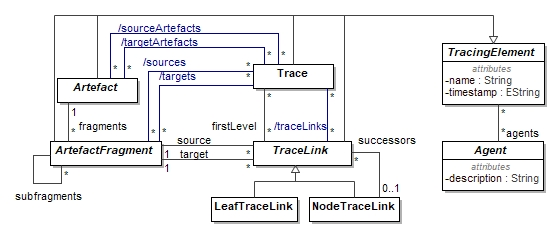
\includegraphics[width=.99\linewidth]{images/core.jpg}
	\caption{Core compositional nature of the Tracea}
	\label{fig:mm-core}
\end{figure}

Based on the previous analysis, we present in this section a new traceability metamodel, called Trace\textit{a}. We aim not to present yet another traceability metamodel but one that learns from and supersedes previous proposals in order to provide a more complete metamodel %\footnote{As any metamodel, OCL constraints \cite{CabotG12} could be used to define additional well-formedness rules.} 
 that also responds  to the requirements made explicit in Section \ref{sec:requirements}. 
%In the course of producing this metamodel, we have tried to be as objective and inclusive as possible. To this extend we use existing knowledge on adaptable traceability which we augment with quality aspects found missing in the literature of the field.
To foster legibility, we have added a simple but complete example of the use of our metamodel to conclude this section.

\subsection{Adaptable and configurable traces} 
 
%As we have seen, there exists many approaches addressing the issue of adaptability. 
In Trace\textit{a}, we start from the common core trace representation in several of the existing metamodels but expand and refine it with a more configurable structure that allows one to define the proper level of granularity. 

\subsubsection{Fine grain tracing structure.} The excerpt in Fig. \ref{fig:mm-core} describes the composition scheme of links into a forest-like structure. Its atomic elements are \texttt{TraceLinks}. A trace link refers to a source and a target \texttt{ArtefactFragment}(see below). It may be a leaf -- which means it has no successor links ; or a node -- which means the trace does not \textit{end} with this link. A \texttt{Tracelink} is a composite of \texttt{LeafTraceLink} and \texttt{LeafTraceNode}. A \texttt{Trace} starts from a set of trace links "\texttt{firstLevel}" that connect to their respective trees. The set of derived \texttt{TraceLinks} from the transitive closure of \texttt{firstLevel} is contained in the reference \texttt{traceLinks}. In the same manner, the set of source and target artefacts and fragments of traces (see blue references in Fig.~\ref{fig:mm-core}) is derived as well (see Listing \ref{lst:ocl}).  \texttt{Trace} and \texttt{TraceLink} are subtypes of \texttt{TracingElement} with a unique identifier (name), a timestamp to address consistency issues (see below), and one or more \texttt{Agent} related. 


\lstset{style=mystyleocl}
\noindent\begin{minipage}[t]{.45\textwidth}
\begin{lstlisting}[frame=tlrb]{Name}
context Trace inv firstLevels:
   self.traceLinks
   ->includesAll(self.firstLevels)
   
context Trace inv sources:
   self.firstLevels
   ->collect(source)
   ->includesAll(self.sources)
   
context Trace inv targets:
   self.tracelinks
   ->collect(target)
   ->includesAll(self.targets)
\end{lstlisting}
\end{minipage}\hfill
\begin{minipage}[t]{.45\textwidth}
\begin{lstlisting}[caption={OCL expressions},frame=tlrb,label=lst:ocl]{Name}
context Trace inv sourceArtefacts:
   self.firstLevels
   ->collect(source)
   ->includesAll(
      self.sourceArtefacts.fragments)
   
context Trace inv targetArtefacts:
   self.tracelinks
   ->collect(target)
   ->includesAll(
      self.targetArtefacts.fragments)
\end{lstlisting}

\end{minipage}

\subsubsection{Adaptable artefacts and relationships.}
Existing traceability works differ a lot in the \textit{kind} of artefacts they target. A unified ontology of traced artefacts has yet emerged but a common approach is to distinguish between the nature of artefacts. \textit{I.e.,} from \textit{text intensive} (\textit{e.g.,} requirements, certification) to \textit{structure intensive} (\textit{e.g.,} source code, test cases).  
In Trace\textit{a}, we specialize \texttt{Artefact} with \texttt{TextArtefact}, \texttt{ModelArtefact}, \texttt{CodeArtefact}, and \texttt{TestArtefact}. 
The list is not exhaustive. These high-level types support the user in defining her own (sub)types. They are anchors to refine artefacts and their fragments at an adequate level of granularity.  

To freely adjust the granularity of the artefacts under scrutiny, Trace\textit{a} suggests the fragmentation of \texttt{Artefact}. An \texttt{ArtefactFragment} defines a part of an artefact that is of interest (\textit{e.g.,} a method in a class; a section in a text document). 
Trace\textit{a} implements a high-level separation for artefacts and relationships. This enables the separate customization of artefact types and the semantic relationships among them. The typing of relationships is versatile and we distinguish two kinds depending on the domain they apply to: \texttt{DomainType} and \texttt{EngineeringType}. In the former, the semantic of the final user (\textit{i.e.,} its domain of application) is targeted. In the latter, the concepts used by engineers or modelers are targeted (the domain of engineering). Same as for the artefact types, relationship types are also expected to be customized \cite{Olive02} when needed.

\Fig{fig:customization} shows an excerpt of the Trace\textit{a} metamodel that focus on aspects related to the adaptability of our approach.
\begin{figure}[ht]   
	\centering  
		\vspace{-0.4truecm}

	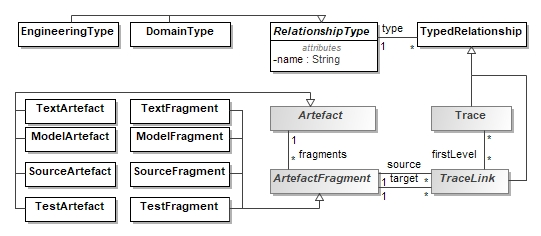
\includegraphics[width=.9\linewidth]{images/customization.jpg}
	\caption{Customization of artefacts and relationships in Tracea}
	\label{fig:customization}
\end{figure}

	\vspace{-0.4truecm}
\subsection{Confidence of trace links}
\begin{figure}[h] 
	\centering
		\vspace{-0.4truecm}

	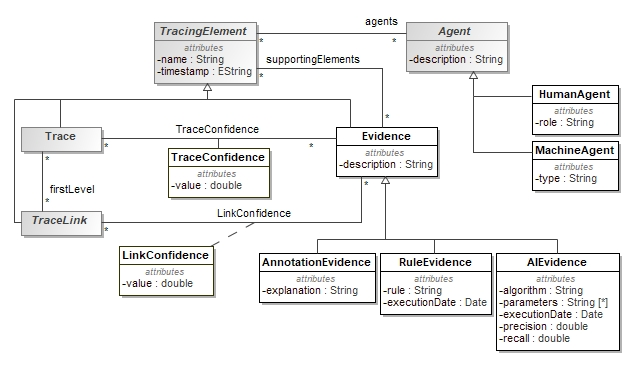
\includegraphics[width=.99\linewidth]{images/explainability.jpg}
	\caption{Representing Explaining traceability with confidence value, agents and evidences}
	\label{fig:explainability}
\end{figure}


In Trace\textit{a}, the confidence of a trace (\texttt{TraceConfidence}) or of a trace link (\texttt{Link- Confidence}) is a statement with a real number value representing the level (from 0 to 1) at which the trace is certain to exist in the system.
It is a statement about the relevance of a trace. A trace and its links are made by \texttt{Agents}. As illustrated in Fig.~\ref{fig:explainability}, an agent may be human (\textit{e.g.,} when traces are elicited manually), or an agent may be a machine (\textit{e.g.,} when an algorithm identify the trace automatically).


\subsection{Trace Consistency}
%\ugh{timestamp: every point knows if it complies with elements. Date comparison. update confidence with finer grain data to consider the decay of tracing artefacts.}
To address the issue of gradual decay, tracing elements must be considered alike with other software artefacts. Their evolution must be scrupulously and synchronously monitored. To be able to represent (and later reason) on the potential decay, we add a timestamp attribute to \texttt{TracingElement} (see Figure \ref{fig:explainability}), \textit{de facto} transforming all metaclasses inheriting from it in temporal elements. We can then use these timestamps to compare the age of a trace compared to the age of the elements traced by it and, if needed, update the confidence we have in that trace, or trace link, accordingly.

%This attribute is not sufficient by itself but assists the integration of tracing elements into version control systems (\textit{e.g.,} Git, SVN), or temporal management system such as TempoEMF.

\subsection{Explainability}
Traces are a key element in many software engineering activities. Therefore, engineers may not want to just take them at \textit{face value} but ask for explanations on how and when the trace was created. Previous subsection covered the \textit{when}, here we focus on the \textit{how}.

The degree of confidence may be justified with evidences, if they exist, to explain the rationale behind the quantitative value. In case of links automatically identified, an evidence instance can record the information necessary to reproduce the identification process or at least to partially explain it. 

More precisely, as can be seen in Fig. \ref{fig:explainability}, an evidence refines into three sub-types: \texttt{AnnotationEvidence} contains a textual description ; \texttt{RuleEvidence} contains a rule (or a set of rules) in a textual field, as well as the execution date ; and \texttt{AIEvidence} contains attributes that will help reproduce the learning scenario, \textit{e.g.,} the kind of algorithm, a reference to the training set and the associated precision and recall the algorithm, and others parameters. An \texttt{Evidence} explanation can also point to other supporting tracing elements. These elements testify, or illustrate the evidence and will be useful for later consistency check.

Every evidence is also optionally endorsed by a set of Human or Machine agents, which further helps in the explainability of the trace beyond the description and attribute values stored in the Evidence object itself.

\subsection{Illustrative example}


In this section, we introduce a simple illustrative example: tracing the impact of a change in the requirements onto their implementation in Java classes. We show through this example the customization of artefacts and relationships, the importance of a quality evaluation, and how we circumvent consequences of using AI-enabled modules for trace identification.
In this example, links are relating requirements to Java classes that undergo modifications. 

 
\subsubsection{Customization of artefacts and relationships}
In this case, a trace aligns two kinds of artefacts: 
\footnotesize\verb" Requirement specification " and \verb" Source class".
\normalsize

These artefacts are too complex to be used at a coarse level of granularity. Java classes may comprise hundreds (or even thousands) of lines of code, requirement specification documents contain hundreds of sections. To address this size issue, a source \texttt{Artefact} (e.g., a class) is decomposed into smaller part (such as methods). In the same manner, specification documents are decomposed into sections. Listing \ref{lst:declare} shows an excerpt of our textual concrete syntax applied to this example where we can see the fragmentation of artefacts. The structure of the traced system is first described with artefacts and fragments sections. For legibility concern, the only kind of relationship in that example is \texttt{Implement}, \textit{i.e.,} a source class \textit{implements} a requirement section. 


\lstset{style=mystyle}
\noindent\begin{minipage}[t]{.45\textwidth}
\begin{lstlisting}[caption={Artefacts, Fragments, Relationships, and Agents declaration},frame=tlrb,label=lst:declare]{Name}
artefacts {
   Requirement r_01 {fragments {sAuth, sLogout}},
   Source Login.java {fragments { mLogin, mLogError, mLogout }},
}
fragments {
   RequirementSection sAuth { },
   RequirementSection sLogout { },
   Method mLogin { },
   Method mLogError { },
   Method mLogOut { },
}
relationshiptypes {
   EngineeringType Implements {},
}
agents {
   HumanAgent 5e8a5T1e4,
   MachineAgent Rd15OUA5RD 
}
\end{lstlisting}
\end{minipage}\hfill
\begin{minipage}[t]{.45\textwidth}
\begin{lstlisting}[caption={Trace instance},frame=tlrb,label=lst:trace]{Name}
Trace ChangeImpact {
   tracelinks {  
      NodeTraceLink link01 { 
         source sAuth
         target mLogin
         successors {link02}
         relationshiptype Implements  
         agents 5e8a5T1e4
      },
      LeafTraceLink link02 { 
         source mLogin
         target mLogError
         relationshiptype Implements  
      },
      LeafTraceLink link03 { 
         source sLogout
         target mLogout
         successors {}
         relationshiptype Implements  
         agents Rd15OUA5RD
         confidence c01
      },
   }
}
\end{lstlisting}
\end{minipage}



The concrete traces are recorded as illustrated in Listing \ref{lst:trace}. A Trace is identifiable by its name and contains trace links whose composition is described through successors. This example is the minimalist expression of a trace. Each and every element is susceptible to refer to an \texttt{Agent} that indicates who and what is the nature of that “who” responsible for the edification of the trace. In our case, \texttt{link\_01} and \texttt{link\_03} have referees.

\subsubsection{Explainability for AI-enabled traceability}
There exists automated evaluation techniques for change impact that predicts which classes are most likely to change. In this scenario, a change in the requirements links to \textit{potentially} impacted classes, and to \textit{actually} modified classes. This distinction shows a distinction in nature of the links themselves. The former is more inclined to suffer a low level of confidence than the automatized latter. In our case, Listing \ref{lst:trace} shows that links \texttt{link\_01} and \texttt{link\_02} have been manually identified, and thus, there the confidence is \texttt{1.0} whereas \texttt{Link\_03} has been automatically suggested and boasts a confidence of \texttt{0.8}.
This level of confidence relies on evidence based on the algorithm employed, its parameterization, and its training setting. As can be seen in Listing \ref{lst:integrity}, a confidence is related to a \texttt{Trace} or a \texttt{TraceLink} and a set of \texttt{Evidence}s. %This representation simplifies the sections in which artefacts, fragments and links are defined. 

Evidences may be an \texttt{AIEvidence} like the one we just described, or \texttt{RuleEvide- nce} that relates patterns used for automatic identification, or \texttt{AnnotationEvidence} that simply contains a textual explanation of the evidence. 
In the example in Listing \ref{lst:integrity}, the confidence \texttt{value} represents the confidence in the prediction that the method \textit{mLogin} is impacted by a change in requirement \texttt{sAuth}. This prediction has been made using a specific algorithm which run settings can be found in the evidences section.

\begin{center}
\noindent\begin{minipage}[t]{.72\textwidth}
\begin{lstlisting}[caption={Confidence, evidence, and agency},frame=tlrb,label=lst:integrity]
confidences {
   Confidence c01 { 
      value 0.8
      evidence {Evidence_link03}
   },
}
evidences {
   AIEvidence Evidence_link03 {
      algorithmUsed "AI4All"
      parameters {"platform:/resource/training/pos_202012"}
      executionDate "20201207-123536"
      trainingResults .8 .7    
      impactedElements ("link02", mLogin, otherMethod) 
   },
}
agency {
   Rd15OUA5RD {Evidence_link03}
}
\end{lstlisting}
\end{minipage}
\end{center}



    \section{Integration and Tool Support}\label{sec:integration}
%\ugh{A robust metamodel for traceability must be able to satisfy different needs and to that purpose shall be conceived in a modular way that allows potential users to take the parts of the metamodel they need in their scenario.}

An Xtext-based\footnote{\url{https://www.eclipse.org/Xtext/}} definition of our metamodel is available on a Git repository\footnote{\url{https://github.com/ebatot/TraceaDSL}}. As concrete syntax, we are using the JSON textual syntax shown in the examples above and illustrated in \Fig{fig:plugin}. 

\begin{figure}[ht] 
	\centering
	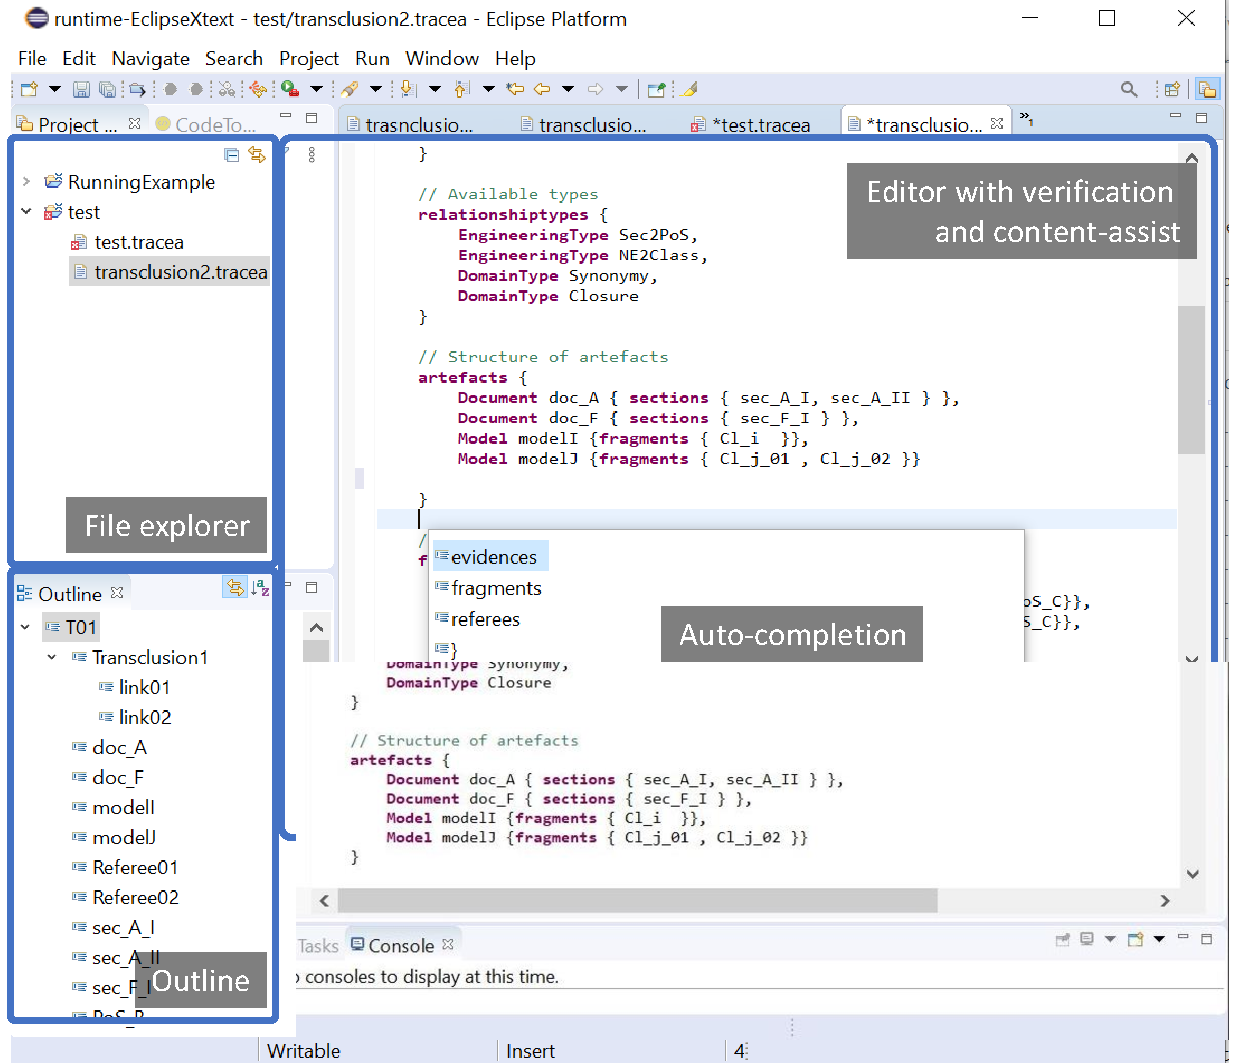
\includegraphics[width=.7\linewidth]{images/plugin-screenshot.pdf}
	\caption{Trace\textit{a} Xtext plugin}
	
	\label{fig:plugin}
\end{figure}


Beyond this option, we have also integrated Trace\textit{a} on top of Capra\footnote{\url{https://projects.eclipse.org/projects/modeling.capra}}. Eclipse Capra is a traceability management tool offering some interesting features to edit and visualize traces, including traceability matrices and graph visualisations. Capra includes a customization language based on Xcore\footnote{\url{https://wiki.eclipse.org/Xcore}}  we have used to add Trace\textit{a} concepts as Capra extensions. %. We employ this mechanism to integrate in the concept of trace link the quality aspects we defined earlier
Thanks to this integration you can benefit from the advanced metamodeling concepts in Trace\textit{a} while also enjoying Capra's visualization capabilities.  

In both cases, the designer can use Trace\textit{a} as a standalone tool or add it as a new component to any model-driven pipeline, especially implemented on top of the EMF Eclipse ecosystem. 

As, in complex scenarios, traces can come from different systems (using different languages or even third-party APIs), it is useful to keep Trace\textit{a} as an \textit{external language} that you can adapt to the changing needs of your application scenario and the types of artefacts you need to trace  \cite{clelandhuang2007bestPracticeForAutomatedTraceability,maro2016_maintenance_factors_and_guidelines}. 

But as a trade-off, this forces designers to learn and add to their toolset a new language. An alternative option is to define Trace\textit{a} as kind of internal DSL, embedded in a more general modeling language like SysML or UML using the extension capabilities offered by them, e.g. UML profiles. 
 
 %Yet, traceability techniques are gaining ground in the engineering of dedicated languages. \textit{E.g.,} IBM Rational DOORS and OMG SysML are built with interfaces for generic traceability -- it is \textit{embedded} in their specification. 


    \section{Conclusion}\label{sec:conclusion}
Traceability research is scattered among different software engineering subfields resulting in diverse but partial solutions to represent traceability information. We have presented a complete traceability metamodel that aims to cover all its aspects, including the quality and uncertainty of specific traces, their decay or the evidences that support them. This information is needed to make fully informed decisions based on trace data. Our proposal has also been designed with modularity and extensibility principles in mind to facilitate its adoption in a large variety of domains. We believe it should help in improving a number of traceability-based algorithms (e.g. for impact change analysis) that could now also take into account these additional traceability dimensions.

As further work we want to continue advancing on these latter aspects, mainly proposing extensions to general modeling languages (like SysML or UML) that integrate our traceability metamodel. Moreover, we will explore the complementarity of AI and traceability. Regarding AI for traceability detection we plan to extend existing techniques to automatically infer traces to populate our metamodel considering the integrity and quality aspects of the inference process. Regarding traceability for AI, we plan to rely on our metamodel to offer better explainability support to the myriad of AI-based solutions for Software Engineering that right now mostly ignore this aspect~\cite{carleton2020-intersection-AI-and-SE,ozkaya2020-differences-in-AI-enabled-engineering}.
%We will study the application of this metamodel to AI applications in software engineering and its integration in general purpose modeling languages, like SysML, as hinted above.
    %\subsection{Illustrative example}


In this section, we introduce a simple illustrative example: tracing the impact of a change in the requirements onto their implementation in Java classes. We show through this example the customization of artefacts and relationships, the importance of a quality evaluation, and how we circumvent consequences of using AI-enabled modules for trace identification.
In this example, links are relating requirements to Java classes that undergo modifications. 

 
\subsubsection{Customization of artefacts and relationships}
In this case, a trace aligns two kinds of artefacts: 
\footnotesize\verb" Requirement specification " and \verb" Source class".
\normalsize

These artefacts are too complex to be used at a coarse level of granularity. Java classes may comprise hundreds (or even thousands) of lines of code, requirement specification documents contain hundreds of sections. To address this size issue, a source \texttt{Artefact} (e.g., a class) is decomposed into smaller part (such as methods). In the same manner, specification documents are decomposed into sections. Listing \ref{lst:declare} shows an excerpt of our textual concrete syntax applied to this example where we can see the fragmentation of artefacts. The structure of the traced system is first described with artefacts and fragments sections. For legibility concern, the only kind of relationship in that example is \texttt{Implement}, \textit{i.e.,} a source class \textit{implements} a requirement section. 


\lstset{style=mystyle}
\noindent\begin{minipage}[t]{.45\textwidth}
\begin{lstlisting}[caption={Artefacts, Fragments, Relationships, and Agents declaration},frame=tlrb,label=lst:declare]{Name}
artefacts {
   Requirement r_01 {fragments {sAuth, sLogout}},
   Source Login.java {fragments { mLogin, mLogError, mLogout }},
}
fragments {
   RequirementSection sAuth { },
   RequirementSection sLogout { },
   Method mLogin { },
   Method mLogError { },
   Method mLogOut { },
}
relationshiptypes {
   EngineeringType Implements {},
}
agents {
   HumanAgent 5e8a5T1e4,
   MachineAgent Rd15OUA5RD 
}
\end{lstlisting}
\end{minipage}\hfill
\begin{minipage}[t]{.45\textwidth}
\begin{lstlisting}[caption={Trace instance},frame=tlrb,label=lst:trace]{Name}
Trace ChangeImpact {
   tracelinks {  
      NodeTraceLink link01 { 
         source sAuth
         target mLogin
         successors {link02}
         relationshiptype Implements  
         agents 5e8a5T1e4
      },
      LeafTraceLink link02 { 
         source mLogin
         target mLogError
         relationshiptype Implements  
      },
      LeafTraceLink link03 { 
         source sLogout
         target mLogout
         successors {}
         relationshiptype Implements  
         agents Rd15OUA5RD
         confidence c01
      },
   }
}
\end{lstlisting}
\end{minipage}



The concrete traces are recorded as illustrated in Listing \ref{lst:trace}. A Trace is identifiable by its name and contains trace links whose composition is described through successors. This example is the minimalist expression of a trace. Each and every element is susceptible to refer to an \texttt{Agent} that indicates who and what is the nature of that “who” responsible for the edification of the trace. In our case, \texttt{link\_01} and \texttt{link\_03} have referees.

\subsubsection{Explainability for AI-enabled traceability}
There exists automated evaluation techniques for change impact that predicts which classes are most likely to change. In this scenario, a change in the requirements links to \textit{potentially} impacted classes, and to \textit{actually} modified classes. This distinction shows a distinction in nature of the links themselves. The former is more inclined to suffer a low level of confidence than the automatized latter. In our case, Listing \ref{lst:trace} shows that links \texttt{link\_01} and \texttt{link\_02} have been manually identified, and thus, there the confidence is \texttt{1.0} whereas \texttt{Link\_03} has been automatically suggested and boasts a confidence of \texttt{0.8}.
This level of confidence relies on evidence based on the algorithm employed, its parameterization, and its training setting. As can be seen in Listing \ref{lst:integrity}, a confidence is related to a \texttt{Trace} or a \texttt{TraceLink} and a set of \texttt{Evidence}s. %This representation simplifies the sections in which artefacts, fragments and links are defined. 

Evidences may be an \texttt{AIEvidence} like the one we just described, or \texttt{RuleEvide- nce} that relates patterns used for automatic identification, or \texttt{AnnotationEvidence} that simply contains a textual explanation of the evidence. 
In the example in Listing \ref{lst:integrity}, the confidence \texttt{value} represents the confidence in the prediction that the method \textit{mLogin} is impacted by a change in requirement \texttt{sAuth}. This prediction has been made using a specific algorithm which run settings can be found in the evidences section.

\begin{center}
\noindent\begin{minipage}[t]{.72\textwidth}
\begin{lstlisting}[caption={Confidence, evidence, and agency},frame=tlrb,label=lst:integrity]
confidences {
   Confidence c01 { 
      value 0.8
      evidence {Evidence_link03}
   },
}
evidences {
   AIEvidence Evidence_link03 {
      algorithmUsed "AI4All"
      parameters {"platform:/resource/training/pos_202012"}
      executionDate "20201207-123536"
      trainingResults .8 .7    
      impactedElements ("link02", mLogin, otherMethod) 
   },
}
agency {
   Rd15OUA5RD {Evidence_link03}
}
\end{lstlisting}
\end{minipage}
\end{center}



%\bibliographystyle{utils/spbasic}      % basic style, author-year citations
\bibliographystyle{utils/splncs04}      % basic style, author-year citations


%\bibliographystyle{spbasic}      % basic style, author-year citations
%\bibliographystyle{spmpsci}      % mathematics and physical sciences
%\bibliographystyle{spphys}       % APS-like style for physics
%\bibliographystyle{utils/plainnatnourl}
%\setcitestyle{numbers}
\bibliography{bib/strings-abbr,bib/uoc2021_traceaMM,bib/added,bib/trace-and-models}


\end{document}
